\documentclass[12pt] {article}
\usepackage{graphicx}
\usepackage{natbib}
\usepackage{fullpage}
\usepackage{amsmath}
\PassOptionsToPackage{hyphens}{url}\usepackage{hyperref}
\usepackage{pslatex}
\renewcommand{\baselinestretch}{2}


\begin{document}
\title{Manual of Best Practices in Transparent Social Science Research}

\author{Garret Christensen\thanks{Berkeley Initiative for Transparency in the Social Sciences, Center for Open Science}}
\date{\today}
\maketitle
\newpage
\tableofcontents

\newpage
\section{Introduction}\label{introduction}

Scientific claims should be subject to scrutiny by other researchers and
the public at large. An essential requirement for such scrutiny is that
researchers make their claims transparent in a way that other
researchers are able to use easily available resources to form a
complete understanding of the methods that were used by the original. In
the social sciences, especially given the personal computing and
Internet revolutions and the wide availability of data and processing
power, it is essential that data, code, and analyses be transparent.

This manual is intended to be a source mainly for empirical social
science researchers who desire to make their own research transparent
to, and reproducible by, others. The entire process of research, from
hypothesis generation to publication, is covered. Although norms differ
across disciplines, we attempt to bring a broad view of the empirical
social sciences to these recommendations, and hope that students and
researchers in any social science field may tailor these recommendations
to best fit their field.

In section~\ref{ethical-research} we first discuss the motivation for this document: the
desire to do ethical research. A major component of ethical social
science research is treating research subjects appropriately. This is
mandated by federal law and overseen by Institutional Review Boards
(IRBs), and should be taken seriously by researchers. But just as
treating subjects fairly is ethical, we believe that transparent,
reproducible research is also a major part of ethical research.

In section~\ref{study-design} we discuss study design, including how to power studies
appropriately.

In section~\ref{registration} we discuss one of the major problems in non-transparent
research, specifically publication bias. We also discuss how this
problem can be resolved through the practice of registration.
Publication bias stems from the fact that published results are
overwhelmingly statistically significant. But without knowing how many
tests were run, it is impossible to know whether these significant
results are meaningful, or whether they are the 5\% of tests that we
would expect to appear significant due to random sampling, even with no
true effect. By publicly registering all studies, we can have a better
idea of just how many tests have been run.

In section~\ref{rdof} we discuss researcher degrees of freedom and pre-analysis
plans; In addition to registering trials, researchers should also
specify their outcomes of interest and their exact methods of analysis
to bind their hands during the analysis phase by writing a Pre-Analysis
Plan (PAP). This is a relatively new idea in the social sciences, so
there is not yet a consensus on when a PAP should be required, what the
ideal level of detail is, and how much it should constrain the
researchers hand in the actual analysis, but by pre-specifying analyses,
researchers can distinguish between confirmatory and exploratory
analysis. We do not necessarily place higher intrinsic value on one or
the other, but making the distinction clear is key for appropriate
interpretation.

In section~\ref{replication-and-reproducibility} we discuss workflow and materials sharing, with an eye on
making research replicable by others. Researchers should make their code
and data publicly available so that others may repeat and verify their
analysis. Making data available incentivizes researchers to make their
work accurate in the first place, and makes replication easier for
others, improving the scientific process, but also raises the concern of
differential privacy, since steps should be taken to prevent
identification of individuals in the data. We also discuss the issue of
reporting standards: a standardized list of things that authors should
report to help make their work reproducible.

Section~\ref{conclusion} concludes.

%%%%%%%%%%%%%%%%%%%%%%%%%%%%%%%%%%%
\section{Ethical Research}\label{ethical-research}

We believe that making one's research transparent and reproducible is a
key component of ethical research.

\subsection{Fraud}\label{fraud}

While most of us are likely to presume that we ourselves would not
conduct outright fraud, fraud does indeed occur. From making up fake
data to creating bogus e-mail addresses so one could do one's own peer
review, the Retraction Watch blog (\url{http://www.retractionwatch.com})
documents a distressingly large amount of deliberate fraud in research.
Although the blog tends to specialize in the life sciences, there is no
good reason to believe that social science researchers are inherently
more benevolent. Part of the US Department of Health and Human Services
, the Office of Research Integrity (ORI), works to promote research
integrity and document misconduct, especially when it involves federally
funded research. The misconduct case summaries of the ORI
(\url{http://ori.hhs.gov/case_summary}), and the stories of Diederik
Stapel (Bhattacharjee 2013; Carey 2011) Hwang Woo-Suk (Cyranoski 2014)
and Marc Hauser (Johnson 2012) should be sobering warnings to us all.

\subsection{Unintentional Bias}\label{unintentional-bias}

Perhaps in addition to the obvious need to avoid deliberate fraud and
protect our human subjects is the need to avoid subconsciously biasing
our own results.

Nosek, Spies, and Motyl (2012) summarize some of the evidence on this
subject, concluding that there are many circumstances common to academia
and the publishing paradigm that cause researchers to frequently use
motivated reasoning:

\begin{quote}
Because we have directional goals for success, we are likely to bring to
bear motivated reasoning to justify research decisions in the name of
accuracy, when they are actually in service of career advancement
(Fanelli, 2010a). Motivated reasoning is particularly influential when
the situation is complex, the available information is ambiguous, and
legitimate reasons can be generated for multiple courses of action
(Bersoff, 1999; Boiney, Kennedy, \& Nye, 1997; Kunda, 1990).

Motivated reasoning can occur without intention. We are more likely to
be convinced that our hypothesis is true, accepting uncritically when it
is confirmed and crutinizing heavily when it is not (Bastardi, Uhlmann,
\& Ross, 2011; Ditto \& Lopez, 1992; Lord, Ross, \& Lepper, 1979;
Pyszczynski \& Greenberg, 1987; Trope \& Bassok, 1982). With flexible
analysis options, we are more likely to find the one that produces a
more publishable pattern of results to be more reasonable and defensible
than others (Simmons et al., 2011; Wagenmakers, Wetzels, Borsboom, \&
van der Maas, 2011). Once we obtain an unexpected result, we are likely
to reconstruct our histories and perceive the outcome as something that
we could have, even did, anticipate all along---converting a discovery
into a confirmatory result (Fischoff, 1977; Fischoff \& Beyth, 1975).
And even if we resist those reasoning biases in the moment, after a few
months, we might simply forget the details, whether we had hypothesized
the moderator, had good justification for one set of exclusion criteria
compared with another, and had really thought that the one dependent
variable that showed a significant effect was the key outcome. Instead,
we might remember the gist of what the study was and what we found
(Reyna \& Brainerd, 1995). Forgetting the details provides an
opportunity for reimagining the study purpose and results to recall and
understand them in their best (i.e., most publishable) light. The reader
may, as we do, recall personal examples of such motivated
decisions---they are entirely ordinary products of human cognition.
\end{quote}

\subsection{Institutional Review
Boards}\label{institutional-review-boards}

In addition to fraud, a major ethical concern relates to our human
subjects.

\subsubsection{History}\label{history}

World history is rife with examples of atrocities conducted in the name
of research. Some of these have resulted in major changes in regulations
related to research.

\paragraph{Nuremberg}\label{nuremberg}

Nazi German doctors conducted horrible experiments on subjects during
World War II. The ``Doctor's Trial'' (USA v. Karl Brandt, et al.) tried
23 defendants, and the verdict included the following ten principles,
which although never entered as formal regulations in either Germany or
the USA, became widely accepted.

\begin{enumerate}
\def\labelenumi{\arabic{enumi}.}
\item
  The voluntary consent of the human subject is absolutely essential.

  This means that the person involved should have legal capacity to give
  consent; should be so situated as to be able to exercise free power of
  choice, without the intervention of any element of force, fraud,
  deceit, duress, over-reaching, or other ulterior form of constraint or
  coercion; and should have sufficient knowledge and comprehension of
  the elements of the subject matter involved as to enable him to make
  an understanding and enlightened decision. This latter element
  requires that before the acceptance of an affirmative decision by the
  experimental subject there should be made known to him the nature,
  duration, and purpose of the experiment; the method and means by which
  it is to be conducted; all inconveniences and hazards reasonably to be
  expected; and the effects upon his health or person which may possibly
  come from his participation in the experiment.

  The duty and responsibility for ascertaining the quality of the
  consent rests upon each individual who initiates, directs or engages
  in the experiment. It is a personal duty and responsibility which may
  not be delegated to another with impunity.
\item
  The experiment should be such as to yield fruitful results for the
  good of society, unprocurable by other methods or means of study, and
  not random and unnecessary in nature.
\item
  The experiment should be so designed and based on the results of
  animal experimentation and a knowledge of the natural history of the
  disease or other problem under study that the anticipated results will
  justify the performance of the experiment.
\item
  The experiment should be so conducted as to avoid all unnecessary
  physical and mental suffering and injury.
\item
  No experiment should be conducted where there is an a priori reason to
  believe that death or disabling injury will occur; except, perhaps, in
  those experiments where the experimental physicians also serve as
  subjects.
\item
  The degree of risk to be taken should never exceed that determined by
  the humanitarian importance of the problem to be solved by the
  experiment.
\item
  Proper preparations should be made and adequate facilities provided to
  protect the experimental subject against even remote possibilities of
  injury, disability, or death.
\item
  The experiment should be conducted only by scientifically qualified
  persons. The highest degree of skill and care should be required
  through all stages of the experiment of those who conduct or engage in
  the experiment.
\item
  During the course of the experiment the human subject should be at
  liberty to bring the experiment to an end if he has reached the
  physical or mental state where continuation of the experiment seems to
  him to be impossible.
\item
  During the course of the experiment the scientist in charge must be
  prepared to terminate the experiment at any stage, if he has probably
  cause to believe, in the exercise of the good faith, superior skill
  and careful judgment required of him that a continuation of the
  experiment is likely to result in injury, disability, or death to the
  experimental subject.
\end{enumerate}

\paragraph{Tuskegee and US
codification}\label{tuskegee-and-us-codification}

In 1972 whistleblower Peter Buxton revealed to the Associated Press that
the US Public Health Service was conducting a 40-year experiment on poor
Alabama sharecroppers in which it did not treat those who had syphilis
for the disease despite the discovery and verification of penicillin as
an effective treatment, and actually prevented sufferers from obtaining
treatment elsewhere. As a result, the National Commission for the
Protection of Human Subjects of Biomedical and Behavioral Research was
formed by law in 1974, and released the Belmont Report in 1979. The
Belmont Report, available at
\url{http://www.hhs.gov/ohrp/humansubjects/guidance/belmont.html},
contains three basic ethical principles, and three applications:

\begin{itemize}
\item
  Ethical Principles

  \begin{itemize}
  \item
    Respect for Persons: ``Respect for persons incorporates at least two
    ethical convictions: first, that individuals should be treated as
    autonomous agents, and second, that persons with diminished autonomy
    are entitled to protection.''
  \item
    Beneficence: ``Two general rules have been formulated as
    complementary expressions of beneficent actions in this sense:
    \textbf{(1)} do not harm and \textbf{(2)} maximize possible benefits
    and minimize possible harms.''
  \item
    Justice: ``An injustice occurs when some benefit to which a person
    is entitled is denied without good reason or when some burden is
    imposed unduly. Another way of conceiving the principle of justice
    is that equals ought to be treated equally.''
  \end{itemize}
\item
  Applications

  \begin{itemize}
  \item
    Informed Consent: ``Respect for persons requires that subjects, to
    the degree that they are capable, be given the opportunity to choose
    what shall or shall not happen to them. This opportunity is provided
    when adequate standards for informed consent are satisfied.''
  \item
    Assessment of Risks and Benefits: ``It is commonly said that
    benefits and risks must be''balanced" and shown to be ``in a
    favorable ratio.'' The metaphorical character of these terms draws
    attention to the difficulty of making precise judgments. Only on
    rare occasions will quantitative techniques be available for the
    scrutiny of research protocols. However, the idea of systematic,
    nonarbitrary analysis of risks and benefits should be emulated
    insofar as possible."
  \item
    Selection of Subjects: ``Individual justice in the selection of
    subjects would require that researchers exhibit fairness: thus, they
    should not offer potentially beneficial research only to some
    patients who are in their favor or select only''undesirable" persons
    for risky research. Social justice requires that distinction be
    drawn between classes of subjects that ought, and ought not, to
    participate in any particular kind of research, based on the ability
    of members of that class to bear burdens and on the appropriateness
    of placing further burdens on already burdened persons."
  \end{itemize}
\end{itemize}

In 1981 the Department of Health and Human Services and the Food and
Drug Administration adopted regulations in line with the Belmont report,
and 15 federal agencies adopted these regulations (45 CFR part 46) as
the ``Common Rule'' in 1991. See
\url{http://www.hhs.gov/ohrp/index.html} for more information.

In practice, this means that researchers who receive funding from the US
government, or who work at institutions that receive federal funding
(i.e.~essentially all researchers) should have their research approved
by an Institutional Review Board (IRB). IRB are a decentralized approval
body set up by each research organization itself, consisting of at least
five members, a mix of men and women, scientists and non-scientists, and
at least one member not affiliated with the institution. Since IRBs and
the approval process are decentralized, the exact process varies from
institution to institution, but one example can be seen at
\url{http://cphs.berkeley.edu}.

When conducting research internationally, researchers should give their
human subjects the same protections as those inside the US. Laws in
developing countries may not be as well-defined or enforced, but
researchers should still register with their US institution's IRB, and
obtain approval from the host country government. A list of laws and
regulations that cover research in 107 foreign countries is available
from the Office for Human Research Protections at
\url{http://www.hhs.gov/ohrp/international/intlcompilation/2014intlcomp.pdf.pdf}.

Another key resource for researchers and research conducted outside the
US is the Declaration of Helsinki by the World Medical Association
(WMA), available at
\url{http://www.wma.net/en/30publications/10policies/b3/index.html}.
Originally adopted by the WMA in 1964, the document has significantly
influenced the laws and regulations adopted to govern research
worldwide.

Lest one think that ethical concerns are limited to monsters of bygone
eras, we refer readers to a dilemma caused by an election experiment by
researchers from Stanford and Dartmouth in 2014:
\url{http://www.washingtonpost.com/blogs/monkey-cage/wp/2014/11/03/ethics-and-research-in-comparative-politics/}.

\subsubsection{Training}\label{training}

A large number of universities participate in the Collaborative
Institutional Training Initiative at the University of Miami (CITI,
\url{https://www.citiprogram.org/}). Completing their course on Human
Subjects Research is often a requirement of being included on a research
proposal.
%%%%%%%%%%%%%%%%%%%%%%%%%%%%%%%%%%%%%
\section{Study Design}\label{study-design}
%Courtney to add this section

%%%%%%%%%%%%%%%%%%%%%%%%%%%%%%%%%%%%%%%%
\section{Registration}\label{registration}

One of the problems brought into focus recently is publication bias.
Publication bias is the selective publication of only significant
results. Thankfully, there are tools available for researchers to combat
these problems.

\subsection{Publication Bias}\label{publication-bias}

One of the primary drivers of the recent move towards transparency is
increased awareness of publication bias. Numerous papers use collections
of published papers to show that the proportion of significant results
are extremely unlikely to come from any true population distribution
(DeLong and Lang 1992; A. S. Gerber, Green, and Nickerson 2001; J. P. A.
Ioannidis 2005). By examining the publication rates of null results and
significant results from a large set of NSF-funded studies, Franco,
Malhotra, and Simonovits (2014) show that the publication of only
significant results may stem from the fact that social science
researchers largely fail to write up and submit results from studies
resulting in null findings, citing lack of interest or fear of
rejection. In fact, the percentage of null findings published in
journals appeas to have been decreasing over time, across all
disciplines (Fanelli 2012). Clearly, there is no reason why this would
be an accurate reflection of the state of the universe. If journals only
publish statistically significant results, we have no idea how many of
those significant results are evidence of real effects, and which are
the 5\% of random draws that we should expect to show a significant
result with a true zero effect. One way to combat this problem is to
require registration of all studies undertaken. Ideally we then search
the registry for studies of X on Y. If numerous studies all show an
effect, we have confidence the effect is real. If 5\% of studies show a
significant effect, we give the outlier study less credence.

\subsection{Trial Registration}\label{trial-registration}

A basic definition of registration is to publicly declare \emph{all}
research that one plans on conducting. Ideally this is done in a public
registry designed to accept registries in the given research discipline,
and ideally the registration takes place before data collection begins.

Almost all registration efforts have thus far been limited to randomized
control trials, as opposed to observational data. (However, we believe
that registering all types of analysis would be ideal.) Registration of
randomized trials has achieved wide adoption in medicine, but is still
relatively new to the social sciences. After congress passed a law in
1997 requiring the creation of a registry for FDA-regulated trials, and
the NIH created clinicaltrials.gov in 2000, The International Committee
of Medical Journal Editors (ICMJE), a collection of editors of top
medical journals, instituted a policy of publishing only registered
trials in 2005 (De Angelis et al. 2004), and the policy has spread to
other journals and been generally accepted by researchers (Laine et al.
2007).

A profound example of the benefit of trial registries is detailed in
Turner et al. (2008), which details the publication rates of studies
related to FDA-approved antidepressants. (See also Ioannidis (2008).)
The outcome is perhaps what the most hardened cynic would expect:
essentially all the trials with positive outcomes were published, a
50/50 mix of questionable studies were published, and a majority of the
negative studies were unpublished a minimum of four years after the
study was completed. The figure below shows the drastically different
rates of publication, and a large amount of publication bias.
\begin{center}
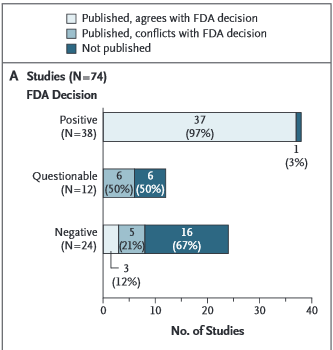
\includegraphics{TurnerFigure1.PNG}

Panel A of Figure 1 from (Turner et al. 2008)
\end{center}
Of course for this sort of exercise to be possible, unless a reader
merely assumes that a registered trial without an associated published
paper produced a null result, it requires that the registration site
itself obtain outcomes of trials. ClinicalTrials.gov is the only
publicly available trial registry that requires such reporting of
results, and only for certain FDA trials.\footnote{HHS and NIH took steps in November 2014 to expand the amount of results reporting required. See \url{http://www.nih.gov/news/health/nov2014/od-19.htm}}  Hartung et al. (2014) raises
concerns about discrepancies between reporting of outcomes in published
papers and in the ClinicalTrials.gov database; as many as 20\% of
studies had discrepancies in primary outcomes and as many as 33\% had
discrepancies in reporting of adverse events.

Even with dramatic growth in medical trial registration, problems
remain. Not all journals have adopted the ICMJE policy, and complete
enforcement is elusive. Mathieu S et al. (2009) looked at trials related
to three medical conditions and found that only 46\% of studies were
registered before the end of the trial with primary outcomes clearly
specified. Even among those adequately registered, 31\% showed some
discrepancies between registered and published outcomes, with bias in
favor of statistically significant definitions.

\subsection{Social Science Registries}\label{social-science-registries}

Registries in the social sciences are newer but are growing ever more
popular. The Abdul Latif Jameel Poverty Action Lab began hosting a
hypothesis registry
(\url{http://www.povertyactionlab.org/hypothesis-registry}) in 2009,
which was superseded by the American Economic Association's launch of
its own registry for randomized trials
(\href{http://www.socialscienceregistry.org}{www.socialscienceregistry.org})
in May 2013, which had accumulated 260 studies in 59 countries by
October 2014. The International Initiative for Impact Evaluation (3ie)
launched its own registry for evaluations of development programs, the
Registry for International Development Impact Evaluations (RIDIE,
\url{http://ridie.3ieimpact.org}) in September 2013, which had
approximately 30 evaluations registered in its first year.

In political science, EGAP: Experiments in Governance and Politics has
created a registry as ``an unsupervised stopgap function to store
designs until the creation of a general registry for social science
research. The EGAP registry focuses on designs for experiments and
observational studies in governance and politics.''
(\url{http://e-gap.org/design-registration}) EGAP's registry had 93
designs registered as of October 2014.\footnote{Other less-widely
  adopted attempts to create registries in political science are the
  Political Science Registered Studies Dataverse (PSRSD,
  \href{../customXml/item1.xml}{http://spia.uga.edu/faculty\_pages/monogan/registration.php})
  and the PAP Registry of the Experimental Research section of the
  American Political Science Association
  (\href{numbering.xml}{http://ps-experiments.ucr.edu/browser}).}

Another location for registrations is the \href{http://osf.io}{Open Science Framework} (OSF), created by the \href{http://centerforopenscience.org/}{Center for Open Science}. The OSF serves as a broad research management tool that encourages and facilitates transparency (see Nosek, Spies, and Motyl (2012).) Registrations are simply unalterable snapshots of research frozen in time, with a persistent URL and timestamp. Researchers can upload their data, code, hypotheses, etc. to the OSF, register it, and then share the resulting URL as proof of registration. OSF registrations can be relatively free-form, but templates exist to conform to standards in different disciplines. Psychology registrations are presently the most numerous on the OSF (\hyperref[newPublicRegistrations]{https://osf.io/explore/activity/\#newPublicRegistrations}).

%%%%%%%%%%%%%%%%%%%%%%%%%%%%%%%%%%%%%%%%%%%%%%%%%%%
\section{Researcher Degrees of
Freedom}\label{rdof}

In addition to publication bias, a problem with research is
specification searching: the manipulation of statistical or regression
models unknowingly (or deliberately) until significance is obtained.
Though registration helps solve the problem of publication bias, it does
not solve the problem of fishing for statistical significance within a
given study. Simmons, Nelson, and Simonsohn (2011) refer to this as
``researcher degrees of freedom,'' and it has also been referred to as
``fishing'' or ``p-hacking.'' Using flexibility around when to stop
collecting data, excluding certain observations, combining and comparing
certain conditions, including certain control variables, and combining
or transforming certain measures, they ``prove'' that listening to the
Beatles' song ``When I'm Sixty-Four'' made listeners a year and a half
younger. The extent and ease of this ``fishing'' is also described in
(Humphreys, Sierra, and Windt 2013). Gelman and Loken (2013) agree that
``{[}a{]} dataset can be analyzed in so many different ways (with the
choices being not just what statistical test to perform but also
decisions on what data to exclude or exclude, {[}sic{]} what measures to
study, what interactions to consider, etc.), that very little
information is provided by the statement that a study came up with a
\emph{p}\textless{}.05 result.'' However, they also conclude that:

\begin{quote}
the term ``fishing" was unfortunate, in that it invokes an image of a
researcher trying out comparison after comparison, throwing the line
into the lake repeatedly until a fish is snagged. We have no reason to
think that researchers regularly do that. We think the real story is
that researchers can perform a reasonable analysis given their
assumptions and their data, but had the data turned out differently,
they could have done other analyses that were just as reasonable in
those circumstances.

We regret the spread of the terms ``fishing" and ``p-hacking'' (and even
``researcher degrees of freedom'') for two reasons: first, because when
such terms are used to describe a study, there is the misleading
implication that researchers were consciously trying out many different
analyses on a single data set; and, second, because it can lead
researchers who know they did not tryout many different analyses to
mistakenly think they are not so strongly subject to problems of
researcher degrees of freedom."
\end{quote}

In other words, the problem is even worse than you think. What can be
done to solve it? We believe part of the answer lies in detailed
pre-analysis plans, described in detail below.

\subsection{Pre-Analysis
Plans}\label{pre-analysis-plans}

While registration of studies can help to reduce publication bias or the file drawer problem, 
A pre-analysis plan (PAP), a detailed outline of the analyses that will be conducted in a sutdy, can be used to reduce researcher degrees of freedom. While registration is now the norm in medicine,
registrations, these often do not include
detailed analysis plans. Sometimes
this is because the medical researcher intends to do very little, if
any, structural or economic-type modeling. But even if a researcher
intends only to compare unadjusted means and bootstrap for standard
errors, this should be explicitly stated. In the social sciences, this
simple comparison is sometimes not the end goal of a randomized trial,
so there may be even more value in pre-specification of intended analyses.
In the section below we explain what exactly should go into a pre-analysis plan.

A pre-analysis plan (PAP) contains a specification of the outcomes of the study, as well as a specification
of the methods that will be used to analyze the outcomes (sometimes
referred to as endpoints in the medical literature). By describing the
method(s) of analysis ahead of time, and to some degree tying the hands
of the researcher, we reduce the ability to data mine. Though one
example of this exists in economics from 2001 (Neumark 2001), the idea
is still quite new to the social sciences. The level of detail varies
widely, and the research community is still constructing norms for
incorporating these documents into final analyses and papers.

Suggestions have been made for the detailed contents of these documents.
\cite{glennerster_running_2013} suggest including the following:

\begin{enumerate}
\def\labelenumi{\arabic{enumi}.}
\item
  the main outcome measures
\item
  which outcome measures are primary and which are secondary,
\item
  the precise composition of any families that will be used for mean
  effects analysis,
\item
  the subgroups that will be analyzed,
\item
  the direction of expected impact if we want to use a one-sided test,
  and
\item
  the primary specification to be used for the analysis.
\end{enumerate}

\cite{glennerster_running_2013} also mention the ``tension between
the benefits of the credibility that comes from tying ones hands versus
the benefits of flexibility to respond to unforeseen events and
results.'' Writing a PAP can lend extra credibility to research by making it of a confirmatory nature as opposed to an exploratory nature.
Both types of research are absolutely valuable, but knowing the distinction is important. If some sort of restriction on the data, be it a specific functional form, exclusion of outliers, or an interaction term (subgroup analysis) that terms a null effect for the population into a significant effect for some subgroup, is specified ahead of time based on theory or previous research, this can be considered confirmatory research. Some would say this is if more value than exploratory research: simply running 20 sub-group analyses and finding that one or two are significant. This may be an estimate of a true effect, but should be labeled as exploratory, and future researchers could attempt to confirm this finding by addressing the question of the sub-group specifically. The potential downside to pre-stating hypotheses and analysis plans is that no matter how carefully researchers plan ahead, something truly unexpected can occur. (An example discussed at a recent conference was subjects showing up for an experiment stoned. One example from a field experiment involved fatalities from a lightning strike at a school \citep{kremer2009incentives}. ) This is why, even though we may use the phrase ``bind our hands,'' we advocate that researchers not be punished for conducting research outside the analysis plan. We simply recommend that researchers clearly delineate which analysis was included in the analysis plan, and which was not, so that readers can know what is confirmatory and what is exploratory.


David McKenzie of the World Bank Research Group proposed a list of ten
items that should be included in a PAP, reproduced below. (For more
detail see
\url{http://blogs.worldbank.org/impactevaluations/a-pre-analysis-plan-checklist})

\begin{enumerate}
\item
  Description of the sample to be used in the study
\item
  Key data sources
\item
  Hypotheses to be tested throughout the causal chain
\item
  Specify how variables will be constructed
\item
  Specify the treatment effect equation to be estimated
\item
  What is the plan for how to deal with multiple outcomes and multiple
  hypothesis testing?
\item
  Procedures to be used for addressing survey attrition
\item
  How will the study deal with outcomes with limited variation?
\item
  If you are going to be testing a model, include the model
\item
  Remember to archive it
\end{enumerate}

In their article on researcher degrees of freedom, Simmons, Nelson, and
Simonsohn (2011) suggest the following requirements for authors:

\begin{enumerate}
\def\labelenumi{\arabic{enumi}.}
\item
  Authors must decide the rule for terminating data collection before
  data collection begins and report this rule in the article.
\item
  Authors must collect at least 20 observations per cell or else provide
  a compelling cost-of-data-collection justification.
\item
  Authors must list all variables collected in a study.
\item
  Authors must report all experimental conditions, including failed
  manipulations.
\item
  If observations are eliminated, authors must also report what the
  statistical results are if those observations are included.
\item
  If an analysis includes a covariate, authors must report the
  statistical results of the analysis without the covariate.
\end{enumerate}

There is some question as to when one should write one's pre-analysis plan. ``Before you begin to analyze your data'' seems like the obvious answer, but this should be precisely defined. One could write the PAP before any baseline survey takes place, after any intervention but before endline, or after endline but before analysis has begun. \cite{glennerster_running_2013} has an informative discussion of the relative values of PAP timing. If one writes the PAP before the baseline, this is in some sense the purest, most free from accusations of p-hacking, but one could also miss valuable information. For example, suppose in baseline one learns that the intended outcome question is phrased poorly and elicits high rates of non-response, or that there is very little variation in the answers to a survey question. If the PAP was written after baseline, one could have accounted for this, but at the same time, researchers would also be free to change the scope of their analysis--for example, in the baseline survey of a field experiment designed to increase wages revealed that few of the subjects worked outside the home, the researcher could change the focus of the analysis. This is not necessarily wrong, but it does change the nature of the analysis somewhat.

PAPs could also be written after endline data has been collected but before the investigators have begun to analyze the data. Some have suggested that one could even look at baseline data from the control group only before writing the PAP. We find this problematic, however, since a researcher could learn that the control group had a particularly low or high value of a certain outcome variable, and then choose to include or not include this variable in the analysis as a result. The original research design could have been intended to analyze the increase in secondary school attendance, but looking at the control group, researcher see that the control group had a very high rate of attendance, making a significant difference between control and treatment (the treatment effect) unlikely. Learning this after the experiment has concluded and searching for things that might be easily different between treatment and control is more exploratory than confirmatory. An alternative proposal from Ben Olken at MIT is to remove the treatment status variable from the dataset before looking at the data, which seems to alleviate some of the concerns. However, one could still search for sub-group analyses at this stage. If you parse the outcome data by gender, and males and females have a similar distribution, to find a differential treatment effect by gender would seem unlikely. If male and female had wildly different outcomes, it would seem like a significant interaction is more likely. This seems like exploratory research. 


\subsubsection{Examples}\label{examples}
Examples of pre-analysis plans in the social sciences are relatively rare, but several examples of good published papers resulting from studies with PAP exist. Several of the items below come from the \href{http://www.povertyactionlab.org/Hypothesis-Registry}{J-PAL Hypothesis Registry}; we highlight those that have publicly available final papers. 


\begin{itemize}
\item 
 \cite{casey_reshaping_2012} includes evidence of large-scale field experiment on community driven development projects in Sierra Leone. The analysis finds no significant benefits. Given the somewhat vague nature of the development projects that resulted from the funding, and the wide variety of potential outcomes, finding signficant results would have been relatively easy. In fact, the paper includes an example of how, if they had the latitude to define outcomes without a pre-analysis plan, the authors could have reported large and significantly positive outcomes. The paper also includes a discussion of the history and purpose of pre-analysis plans. The online appendix, available at \url{http://emiguel.econ.berkeley.edu/assets/miguel_research/8/_Appendix__Reshaping_Institutions_-_Evidence__on__Aid__Impacts__Using__a__Pre___Analysis__Plan.pdf},
contains the PAP.


\item 
Oregon expanded its medicare enrollment through a random lottery in 2008, providing researchers with an ideal avenue to evaluate the benefits of enrollment. \cite{finkelstein_oregon_2012, Taubman17012014, doi:10.1056/NEJMsa1212321} show that recipients did not improve in physical health measurements, but were more likely to have insurance, had beter self-reported health outcomes, utilized emergency rooms more, and had better detection and management of diabetes. Pre-analsyis plans from the project are available at the National Bureau of Economics' site devoted to the project: \url{http://www.nber.org/oregon/documents.html} (See, for example, \cite{taubman_oregon_2013, baicker_katherine_oregon_2014}.)


\item
The shoe company Toms funded a rigorous evaluation of its in-kind shoe donation program. Researchers wrote a pre-analysis plan before conducting their research, and found no evidence that shoe donations displace local purchasing of shoes. See \cite{wydick_-kind_2014, katz_elizabeth_pre-analysis_2013}. The PAP is available at \url{http://www.povertyactionlab.org/doc/pre-analysis-planwydick2-12-13pdf}. This is one of many projects that has benefited from a pre-analysis plan because of the involvement of a group with a vested interest, such as a government or corporation.

\item
Researchers from UC San Diego and the World Bank evaluated job training programs run by the Turkish government and found only insignificant improvements and a strongly negative return on investment. See \cite{almeida_impact_2012, vocationalTurkey}. The PAP is available in the J-PAL registry as well as at
\url{http://blogs.worldbank.org/impactevaluations/files/impactevaluations/iskurie_analysisplan_v4a.pdf}).


\item 
Teams led by Ben Olkin have evaluated multiple randomized interventions in Indonesia. The \href{http://www.povertyactionlab.org/evaluation/project-generasi-conditional-community-block-grants-indonesia}{Generasi program} linked community block grants to performance. The PAP are \cite{olken_generasi_2009, olken_generasi_2010} and are available in the J-PAL Hypothesis Registry \url{http://www.povertyactionlab.org/Hypothesis-Registry}. The researchers found health improvement, but no education improvement \cite{olken_indonesias_2010, olken_should_2014}.

\item 
Another project in Indonesia used a field experiment to evaluate different means of poverty targeting for cash transfer programs: proxy-means testing, community-based targeting, and a hybrid. Results show that the proxy-means testing outperformed the other methods by 10\%, but that community members were far more satisfied with the community method. The PAP and final paper are available as \cite{olken_targeting_2009} and \cite{alatas_targeting_2012}

\item
An example from pyschology is a pre-registered replication of an implicit association test. Existing research showed evidence of stronger racial preferences among fertile women. \cite{NosekPreRegistered} failed to reproduce this effect in four tries, suggesting the association is weaker than originally found. The resulting manuscript, as well as the time-stamped registration of the analysis plan, can be found at \url{https://osf.io/g3sca/}
\end{itemize}

Several of the PAP above, and several of the lists of suggestions above involve corrections for multiple hypothesis testing.  (FWER---cite Michael L Anderson
and the Van der Laan SuperLearner papers)

One aspect of PAPs that seems to have taken hold widely in the medical
literature is the aversion to sub-group analysis (``interactions'' to
most economists). An oft-repeated story revolves around the publication
of a study on aspirin after heart attacks. When the editors suggested
including 40 subgroup analyses, the authors relented on the condition
they include some of their own. Gemini and Libras had worse outcomes
when taking aspirin after heart attacks, despite the large beneficial
effects for everyone else. (Described in Schulz and Grimes (2005),
original finding in (ISIS-2 (SECOND INTERNATIONAL STUDY OF INFARCT
SURVIVAL) COLLABORATIVE GROUP 1988)) Whether in a randomized trial or
not, we feel that economists could benefit from reporting the number of
interactions tested, possibly adjusting for multiple hypotheses, and
ideally specifying beforehand the interactions to be tested.

Somewhere in either registration or PAP or protocol---discuss exact
details of randomization.(Bruhn and McKenzie 2009)

and \url{http://e-gap.org/resources/guides/randomization/}

Conceal your randomized assignment so nobody subverts it. (Schulz and
Grimes 2002)

Limit or pre-specify your sub-group analyses/interactions (Schulz and
Grimes 2005)

The original heart attack for libras and Gemini paper: (ISIS-2 (SECOND
INTERNATIONAL STUDY OF INFARCT SURVIVAL) COLLABORATIVE GROUP 1988)


\subsubsection{Project Protocols}\label{project-protocols}

The PAP is similar to, but distinct from, a project protocol. A protocol is a detailed recipe or instruction
manual for others to use to reproduce an experiment. Protocols
are standard in the medical literature, as in all areas of lab science,
but may be less familiar to those used to working with administrative or
observational data. Lab sciences are rife with examples of experiments failing to replicate because of supposedly minor changes such as the brand of bedding in mouse cages or the gender of the laboratory assistant \citep{sorge2014olfactory}. \textit{Nature} has decided to expand its methods section in order to encourage better reporting.\footnote{\url{http://www.nature.com/news/announcement-reducing-our-irreproducibility-1.12852}}
We believe the social sciences would benefit from more careful documentation of methods. When one uses administrative data this can be accomplished by sharing one's data and code so that analysis is transparent. This is discussed below in section~\ref{replication-and-reproducibility}.\footnote{It should be noted that the need for documentation of survey method is not eliminated by using administrative data, the burden simply falls upon the administration.} With original data collection, researchers should provide very detailed descriptions of what exactly they did. A 33-item checklist of suggested items is contained in the \href{http://www.spirit-statement.org/}{SPIRIT} (Standard Protocol Items: Recommendations for Interventional
Trials) statement (see \url{http://www.spirit-statement.org}, Chan et al. 2013), including details on the participants, interventions, outcomes, assignment, blinding, data collection, data management, and statistical methods, among other things. 

 Some medicine and science journals have begun to publish protocols.   While the
advantages of publishing a protocol related to the development of a new
procedure (e.g. ``we have developed a new method of isolating mRNA'')
should be obvious, the advantages of publishing protocols for randomized
trials under way are perhaps less obvious, but still exist. \emph{BioMed
Central} and \emph{BMJ Open}, among others, now publish protocols of
trials planned or ongoing, with the hopes that this will reduce
publication bias, allow patients to see trials in which they might like
to enroll, allow funders and researchers to learn of work underway to
avoid duplication, and to allow readers to compare what research was
originally proposed to what was actually completed. (See
\url{http://www.biomedcentral.com/authors/protocols} and
\url{http://bmjopen.bmj.com/site/about/guidelines.xhtml\#studyprotocols}.)
\emph{BMJ Open} suggests, but does not require, that its published
protocols include the items in the SPIRIT checklist.

Even in published (or otherwise public) protocols, studies have found
important differences between protocols and published results. 60-71\%
of outcomes described in protocols went unreported in the paper while
62\% had major discrepancies between primary outcomes in the protocols
and in the published papers, though there was a relatively even mix of
these discrepancies favoring significant or insignificant results (Chan
A et al. 2004). Another study found that appropriate level of
statistical detail is often lacking in protocols, and there are often
discrepancies between protocols and published results (Saquib, Saquib,
and Ioannidis 2013). 31\% of published papers had some sort of
pre-specified plan for their regression adjustments (i.e.~specifying
which baseline covariates would be controlled for), while 70-74\% of
those that published a design paper or provided a protocol to the
authors, but only 53\% of the plans matched what was published in the
ultimate paper. While there seems to be internal disagreement in both
medicine and the social sciences over the appropriateness of including baseline
control variables in regression analysis of a randomized trial, having
researchers selectively report whatever method gives them the most
significant-seeming results is obviously not the optimal outcome (Bruhn
and McKenzie 2009).

%%%%%%%%%%%%%%%%%%%%%%%%%%%%%%%%%%%
\section{Replication and
Reproducibility}\label{replication-and-reproducibility}

\begin{quote}
``Economists treat replication the way teenagers treat chastity - as an
ideal to be professed but not to be practised.''---Daniel Hamermesh,
University of Texas at Austin Economics
\end{quote}

\begin{quote}
``Reproducibility is just collaboration with people you don't know,
including yourself next week''---Philip Stark, UC Berkeley Statistics
\end{quote}

Replication, in both practice and principle, is a key part of social
science research. We first define what exactly we mean by replication
using the taxonomy developed in Hamermesh (2007) and Hunter (2001).
Replication comes in a few different shapes: pure, statistical, and
scientific.

\begin{itemize}
\item
  Pure: Using the exact same data and the exact same model to see if the
  published results are reproduced exactly.
\item
  Scientific: Using a different sample from a different population, and
  similar, but perhaps not identical model .
\item
  Statistical: Using the same model and underlying population but a
  different sample. In Hamermesh's view, less relevant to economists,
  who are likely to already use as large a sample as is available.
\end{itemize}

Others have described this in terms of a spectrum from full replication
(independent collection of data and re-running analysis) to
reproducibility, where the same data and code are re-used by other
researchers. (Peng 2011) Whatever the terminology used, transparent
research requires making data and code available to other researchers.

\subsection{Code and Workflow}\label{code-and-workflow}

Reproducing research often involves using the exact code and statistical
programming done by the original researcher. To make this possible, code
needs to be both (1) easily available and (2) easily interpretable.
Thanks to several free and easy to use websites described below, code
can easily be made available by researchers without requiring funding or
website hosting. Making code easily interpretable is a more complicated
task, nevertheless, the extra effort spent to make a more manageable
code pays off with large dividends.

\subsubsection{Publicly Sharing Code}\label{publicly-sharing-code}

Once analysis is complete (or even before this stage) researchers should
share their data and code with the public. GitHub
(\url{http://www.github.com}), The Center for Open Science's Open
Science Framework (\url{http://osf.io}), and Harvard University's
Dataverse (\url{http://thedata.org}) are all free repositories for data
and code that include easy to use version control.\footnote{BitBucket
  (\href{styles.xml}{http://www.bitbucket.org}) XXX, and XXX are also
  web services that one can use for free version control and archiving
  of public data and code.} Version control is simply archiving previous
versions of files so that old versions are not lost and can be returned
to if needed. Instead of simply calling one's analysis code
``MyAnalysis.do'' and repeatedly saving over and losing old versions,
and instead of repeatedly changing the file name from
``MyAnalysis.2014.8.13.do'' to ``MyAnalysis.2014.8.14.do'' according to
the date, version control creates different versions of files and can
compare and highlight the differences in version of text files, and
restore the used file to previous conditions if desired. Web services
such as GitHub have the advantage of being ``distributed'' (DVCS) in
that several users can have access simultaneously.

\subsubsection{Managing Workflow}\label{managing-workflow}

Code is just one aspect of a larger structure we refer to as
``workflow'' after Long (2008) and Kirchkamp (?), by which we mean the
combination of data, code, organization, and documentation: everything
from file and variable names to folder organization as well as efficient
and readable programming, and data storage and documentation.

Software:

Although there is a movement by many towards open source software such
as \href{http://www.r-project.org/}{R} and \href{https://www.python.org/}{Python}, we appreciate that many disciplines have long
traditions of using proprietary software such as SAS and STATA, and
learning a new programming language may be an undesirable additional
task in researchers' busy lives. That said, there are several general
coding rules that all researchers should use when organizing and
implementing their analysis, and researchers should strive to make their
work usable by as many others as possible.

Perhaps the most important rule is to write code, don't work by hand. By
that we mean:

\begin{itemize}
\item
  Do not modify data by hand, such as with a spreadsheet. Which is to
  say, don't use Excel.
\item
  Use neither the command line nor drop-down menus nor point-and-click
  options in statistical software.
\item
  Instead, do everything with scripts.
\end{itemize}

The simple reason for this is reproducibility. Modifying data in Excel
or any similar spreadsheet program leaves no record of the changes made
to the data, nor any explanation of the reasoning or timing behind any
changes. Although it may seem easy or quick to do a one-time-only
cleaning of data in Excel, or make ``minor'' changes to get the data
into a format readable by a researcher's preferred statistical software,
unless these changes are written down in excruciating detail, this is
not reproducible by other researchers. It is better to write a code
script that imports the raw data, does all necessary changes, with
comments in the code that explain changes, and saves any intermediate
data sets used in analysis. Then, researchers can share their initial
raw data and their code, and other researchers can reproduce their work
exactly.

Though we understand that a fair amount of research has been done using
pull down menus in SPSS or Stata, we advise against this. A bare minimum
if one insists on going this route is to use the built-in
command-logging features of the software. In Stata, this involves the
`cmdlog' command, in SPSS, this involves the paste button to add to a
syntax.

The ideal is to make everything, including changes like rounding and
formatting, done with scripts. Even downloading of data from websites
can be done through a script. For example, in R, the download.file()
function can be used to save data from a website. (Though of course this
opens the possibility to the data file changing. When reproducing
results from a given dataset is more important than the data from a
specific source, researchers should download their raw dataset once, and
never save over it, instead saving all modified intermediate datasets in
a separate location.) Another extremely important way to prevent
unintentional changes to data is to always set the seed for random
number generators whenever any random numbers are to be used (set.seed()
in R, set seed () in Stata). Additionally, information about the exact
software version used should be included (Stata version 12.x, or use the
session.info() command in R) as well as computer processor and operating
system information. The casual programmer may assume that sophisticated
software would always produce the exact same answer across multiple
versions of software and platforms, but this is not the case.

Organize Your Work:

Don't save output. Just save code and data that generates it.

Think about the entire pipeline. Terry White ``Hit by a bus test''

\subsection{General Worflow
Suggestions:}\label{general-worflow-suggestions}

\begin{itemize}
\item
  Do not use spaces in directory names
\item
  Use ``naming directories'', .i.e.~a directory beginning with ``-'' (so
  that it will appear first alphabetically) inside each directory to
  explain the contents of the above directory.
\item
  Add name, date, and describe contents, as well as updates, to all
  scripting files.
\item
  Keep a research log
\item
  \begin{itemize}
  \item
    Make sure that all .do files are self-contained, do not require data
    in memory, or ideally, certain directory.
  \end{itemize}
\item
  You can never comment too much.
\item
  Indent your code
\item
  \begin{itemize}
  \item
    Once you post/distribute code or data, any changes at all require a
    new file name.
  \end{itemize}
\item
  Separate your cleaning and analysis files; don't make any new vars
  that need saving (or will be used by a different analysis
  file)---better to only create once so you know they're the same.
\item
  Never name a file ``final'' because it won't be.
\item
  Name variables ``male'' instead of ``gender.''
\item
  Use a prefix such as x\_ or temp\_ so you know which files can easily
  be deleted.
\item
  Never change the contents of a variable unless you give it a new name.
\item
  Every variable should have a label.
\end{itemize}

\subsection{Stata-specific
Suggestions}\label{stata-specific-suggestions}

\begin{itemize}
\item
  Use the different missing values (``.a''-``.z'', not exclusively
  ``.'')
\item
  Make sure code always produces same result---set seed and sort/merge
  stable
\item
  Use the version command
\item
  Don't use abbreviations for variables (may become unstable after
  adding variables) or commands
\item
  Avoid using global macros
\item
  Use locals for varlists
\item
  Use `return' command instead of typing in numbers
\item
  If you have a master .do file that calls other .do files, you can run
  multiple log files at the same time (so you have a master .log file)
\item
  Use the label data and notes commands.
\item
  Use the notes command for variables as well.
\item
  Use the datasignature command to run a hash and ensure that data is
  the same as before.
\item
  Use value labels for all categorical variables, but include the
  numerical value in the label.
\item
  Don't use capital in variable names since not all software packages
  are case sensitive.
\item
  Make your files as non-proprietary as possible (use the `saveold'
  command to enable those with earlier versions to use your data. This
  is why trusted repositories are so good--they'll do this for you.)
\end{itemize}

In addition to making code available to the public, the code itself
should be written in a reader-friendly format, referred to as ``Literate
Programming'' introduced in Knuth (1984) and Knuth (1992). The basic
idea is that ``the time is ripe for significantly better documentation
of programs, and that we can best achieve this by considering programs
to be \emph{works of literature}\ldots{}Instead of imagining that our
main task is to instruct a \emph{computer} what to do, let us
concentrate rather on explaining to \emph{human beings} what we want a
computer to do.'' {[}emphasis original{]} Simply put, code should be
written in as simple and easily understood a way as possible, and should
be very well commented, so that researchers other than the original
author can more easily understand the goal of the code.

One tool to make literate (statistical) programming significantly easier
is Knitr (see (Xie 2014; Xie 2013) which is built into R
Studio\footnote{R Studio is a popular free integrated implementation of
  R, available at \href{stylesWithEffects.xml}{http://www.rstudio.com}.}.
Knitr uses R Markdown (a very simple plain text markup language,
described at \url{http://rmarkdown.rstudio.com/}) in which one writes
both code and comments that is automatically spun into an easily read
and shareable HTML, PDF, or MS Word document. These can be posted and
shared for free at RPubs (\url{https://rpubs.com}), an easy to use
hosting service by Rstudio.

ADD EXAMPLE

R MarkdownMarkdownHTML (edit only the first)

\subsection{Sharing Data}\label{sharing-data}

In addition to code, researchers should share their data if at all
possible. Many journals do not require sharing of code, but the number
that do is increasing.

\subsubsection{The JMCB Project and
Economics}\label{the-jmcb-project-and-economics}

In the field of economics, few, if any journals required sharing of data
before ``The Journal of Money, Credit, and Banking Project,'' published
in \emph{The American Economic Review} in 1986 (Dewald, Thursby, and
Anderson 1986). \emph{The Journal of Money, Credit, and Banking} started
the \emph{JMCB Data Storage and Evaluation Project} with NSF funding in
1982, which requested data and code from authors who published in the
journal. With a great deal of research funded by the NSF, it should be
noted that they have long had an explicit policy of expecting
researchers to share their primary data\footnote{``Investigators are
  expected to share with other researchers, at no more than incremental
  cost and within a reasonable time, the primary data, samples, physical
  collections and other supporting materials created or gathered in the
  course of work under NSF grants. Grantees are expected to encourage
  and facilitate such sharing.'' See
  http://www.nsf.gov/bfa/dias/policy/dmp.jsp}. Despite this, and despite
the explicit policy of the \emph{Journal} during the project, at most
only 78\% of authors provided data to the authors within six months
after multiple requests. (This is admittedly an improvement over the
34\% from the control group---those who published before the
\emph{Journal} policy went into effect---who provided data.) Of the
papers that were still under review by the \emph{Journal} at the time of
the requests for data, one quarter did not even respond to the request,
despite the request coming from the same journal considering their
paper! The submitted data was often an unlabeled and undocumented mess.
Despite this, the authors attempted to replicate nine papers, and often
were completely unable to reproduce published results, despite detailed
assistance from the original authors.

Shockingly, nothing much changed with the publication of this important
article. A decade later, in a follow-up piece to the JMCB Project
published in the Federal Reserve Bank of St.~Louis \emph{Review}
(Anderson and Dewald 1994), the authors note that only two economics
journals other than the \emph{Review} itself (\emph{Journal of Applied
Econometrics, Journal of Business and Economic Statistics}) requested
data from authors, and neither requested code. The \emph{JMCB} itself
discontinued the policy of requesting data in 1993, though it resumed
requesting data in 1996. The authors repeated their experiment with
papers presented at the St.~Louis Federal Reserve Bank conference in
1992, and obtained similar response rates as original JMCB Project. The
flagship economics journal, the \emph{American Economic Review} (AER),
did not start requesting data until 2003. Finally, after a 2003 article
showing the nonlinear maximization methods often produce wildly
different estimates across different software packages, that not a
single AER article tested their solution with different software, and
that fully half of queried authors from a chosen issue of the AER,
including a then editor of the journal, failed to comply with the policy
of providing data and code, editor Ben Bernanke made the data and code
policy mandatory in 2005 (McCullough and Vinod 2003; McCullough 2007).

The current data policy from the \emph{American Economic Review} can be
seen here: \url{https://www.aeaweb.org/aer/data.php}. In addition to all
the journals published by the American Economic Association, several top
journals, including \emph{Econometrica, The Journal of Applied
Econometrics, The Journal of Money Credit and Banking, the Journal of
Political Economy, The Review of Economics and Statistics, and the
Review of Economic Studies}, now explicitly require data and code to be
submitted at the time of publication. The AER conducted a review and
found good, but incomplete, compliance (Glandon 2010).

\subsubsection{General Repositories}\label{general-repositories}

The previous section on the \emph{JMCB} describes only a few journals in
one field of the social sciences. Even if the journal to which you
submit your research does not require you to supply them with your code
and data, researchers should still share these things. Though some
repositories, particularly Harvard's Dataverse, seem equipped to handle
data from practically any researcher (a free 1 TB of storage is
standard, with more possible), many repositories specialize. The
Registry of Research Data Repositories (\url{http://www.re3data.org})
has described over 900 data repositories to help you find the right data
repository for your data. A key advantage to using a trusted repository
such as one listed here, in lieu of simply throwing the data up on your
own website or making your Dropbox folder public, is that many of these
repositories will take your data in its proprietary (Stata, SAS, SPSS,
etc.) form, and make it accessible in other formats.

\subsection{Reporting Standards}\label{reporting-standards}
In research, the devil truly is in the details. Whether it is for assessing the validity of a research design or for
attempting to replicate a study, details of what exactly was done must be recorded and made available to other researchers.
The exact details that are relevant will likely differ from field to field, but an increasing number of fields have
produced centralized checklists that describe (in excruciating detail) what disclosure is required of published studies. These checklists are not often published with the paper, but can be submitted with the original article so that reviewers can check that it has been completed. With infinite and easy web storage, researchers can easily post these materials on their website even if journal editors insist on cutting their methods sections for space reasons. 


%MAYBE PUT PROTOCOLS SECTION HERE? Seems like appropriate place for that sort of detail

\subsubsection{Randomized Trials and CONSORT}\label{randomized-trials}
The most widely adopted reporting standard guideline is the Consolidated Standards of Reporting Trials (CONSORT), available at \url{http://www.consort-statement.org}. Parallel to construction of \href{http://clinicaltrials.gov}{clinicaltrials.gov} and registration,
reporting standards evolved, and are now nearly universally adopted for randomized trials published in medical journals, required or requested by reviewers during the review process. This is still in its infancy in the social sciences.

The original CONSORT  was developed in the mid 1990's (Begg C et al. 1996). After five years, research showed that reporting of essential details, as required by the checklist, had significantly increased in journals requiring the standard  (Moher D et al. 2001). The statement was revised in 2001, and simultaneously published in three of the top journals (Moher, Schulz, and Altman 2001). The statement was again revised in 2010 (Schulz et al. 2010) The statement is a 25-item checklist pertaining to the title, abstract, introduction, methods, results, and discussion of the article in question, and seeks to delineate the minimum requirements of disclosure that may not be sufficiently addressed through other measures.

\subsection{Social Science Reporting Standards}\label{soc-sci-standards}
Though a standard akin to CONSORT has not been formally adopted by social science or behavioral science journals, at least as far as we are aware, there have been attempts to do this: In political science, the Experimental Research Section Standards Committee produced a detailed list of items required for disclosure of experiments in political science (A. Gerber et al. 2014). This checklist is available \href{http://www.davidhendry.net/research-supplemental/gerberetal2014-reportingstandards/gerberetal2014-reportingstandards&appendix1.pdf}{here}.\footnote{\url{http://www.davidhendry.net/research-supplemental/gerberetal2014-reportingstandards/gerberetal2014-reportingstandards&appendix1.pdf}}

In economics, one article has highlighted the fact that there is not much discussion of essential features of randomization (how was randomization stratified, if at all? How were control variables determined?), but no standards have been adoped. (Bruhn and
McKenzie 2009)

\subsection{Observational Reporting Standards}\label{observational-standards}
Social science has yet to make a serious push for reporting standards in observational work, but the medical/epidemiological literature has created standards in this type of work, though they are not as widely adopted as CONSORT. Perhaps the most well-known is the STROBE Statement (Strengthening the reporting of observational studies in epidemiology), available at \url{http://www.strobe-statement.org}. STROBE provides checklists for reporting of cohort, case-control, and cross-sectional studies. These standards have been endorsed by approximately 100 journals in the field.\footnote{\url{http://www.strobe-statement.org/index.php?id=strobe-endorsement}}

Medicine has in fact come up with too many checklists to describe them all individually. Acknowledging that every field and type of research is different, the Equator Network (Enhancing the Quality of Transparency of Health Research) serves as an umbrella organization that seeks to keep tabs on all the best reporting standards and help researchers find which reporting standard is most relevant for their research. See \url{http://www.equator-network.org/} for more information.



\subsection{Differential Privacy}\label{differential-privacy}

One important caveat to making data widely available, is that despite
anonymization, in the age of big data, sometimes individual subjects can
easily be identified. Heffetz and Ligett (2014) recount deliberate data
releases by Yahoo! Inc., the Massachusetts state government, and
Netflix, that could easily be used to identify individuals in the data,
despite the absence of direct identifiers such as names or social
security numbers. The problem is that ``de-identification does not
guarantee anonymization.'' This problem is well known in computer science, but solutions are not yet agreed upon, nor widely implemented.


\section{Conclusion}\label{conclusion}

As you may have noticed, many of the activities described in this manual
require extra work. Before you run an experiment, we're telling you to
write down the hypothesis, carefully explain how you are going to test
the hypothesis, write down the very regression analysis you're going to
run, write a detailed protocol of the exact experimental setting, and
then you have to post all of this publicly on the Internet with some
sort of Big Brother organization. Or at least that's one way to look at
it. But we strongly belive these steps are (1) not that difficult once
you get used to them and (2) well worth the reward. You'll get p-values
you can believe in. The next time someone asks you for your data, you
just point them to the website, where they'll download the data and
code, and the code will produce the exact results in the published
paper. The next time you open up a coding file you haven't looked at in
months to make a change suggested by a reviewer, your code will be so
thoroughly commented, you'll know exactly where to go to make the
changes. And the next time you want to extend the analysis of a
published paper, you click the link in the paper and have the data on
your own computer in seconds. Science moves forward.

%%%%%%%%%%%%%%%%%%%%%%%%%%%%%%%%%%%%%
\section{References}\label{references}
\bibliographystyle{plainnat}
\bibliography{Bibliography}

\textbf{References below this text are included manually}

%Change that!
Alatas, Vivi, Abhijit Banerjee, Rema Hanna, Benjamin A Olken, and Julia
Tobias. 2012. ``Targeting the Poor: Evidence from a Field Experiment in
Indonesia.'' \emph{American Economic Review} 102 (4): 1206-40.
doi:10.1257/aer.102.4.1206.

Almeida, Rita, Sarojini Hirshleifer, David McKenzie, Cristobal
Ridao-Cano, and Ahmed Levent Yener. 2012. ``The Impact of Vocational
Training for the Unemployed in Turkey: Pre-Analysis Plan.''
\emph{Poverty Action Lab Hypothesis Registry}, February.
http://www.povertyactionlab.org/sites/default/files/documents/ISKURIE\_AnalysisPlan\_v4.pdf.

Anderson, Richard G., and William G. Dewald. 1994. ``Replication and
Scientific Standards in Applied Economics a Decade after the Journal of
Money, Credit and Banking Project.'' \emph{Federal Reserve Bank of
St.~Louis Review}, no. Nov: 79-83.

Baicker, Katherine, Finkelstein, Amy, and Taubman, Sarah. 2014. ``The
Oregon Health Insurance Experiment: Evidence from Criminal Charges Data,
Analysis Plan,'' NBER Working Paper, , April.
http://www.nber.org/oregon/files/oregon\_hie\_crime\_analysis\_plan.pdf.

Begg C, Cho M, Eastwood S, and et al. 1996. ``Improving the Quality of
Reporting of Randomized Controlled Trials: The Consort Statement.''
\emph{JAMA} 276 (8): 637-39. doi:10.1001/jama.1996.03540080059030.

Bhattacharjee, Yudhijit. 2013. ``Diederik Stapel's Audacious Academic
Fraud.'' \emph{The New York Times}, April 26, sec.~Magazine.
http://www.nytimes.com/2013/04/28/magazine/diederik-stapels-audacious-academic-fraud.html.

Bruhn, Miriam, and David McKenzie. 2009. ``In Pursuit of Balance:
Randomization in Practice in Development Field Experiments.''
\emph{American Economic Journal: Applied Economics} 1 (4): 200-232.
doi:10.1257/app.1.4.200.

Carey, Benedict. 2011. ``Noted Dutch Psychologist, Stapel, Accused of
Research Fraud.'' \emph{The New York Times}, November 2, sec.~Health /
Research.
http://www.nytimes.com/2011/11/03/health/research/noted-dutch-psychologist-stapel-accused-of-research-fraud.html.

Casey, Katherine, Rachel Glennerster, and Edward Miguel. 2012.
``Reshaping Institutions: Evidence on Aid Impacts Using a Preanalysis
Plan*.'' \emph{The Quarterly Journal of Economics} 127 (4): 1755-1812.
doi:10.1093/qje/qje027.

Chan A, Hróbjartsson A, Haahr MT, Gøtzsche PC, and Altman DG. 2004.
``Empirical Evidence for Selective Reporting of Outcomes in Randomized
Trials: Comparison of Protocols to Published Articles.'' \emph{JAMA} 291
(20): 2457-65. doi:10.1001/jama.291.20.2457.

Chan, A.-W., J. M. Tetzlaff, P. C. Gotzsche, D. G. Altman, H. Mann, J.
A. Berlin, K. Dickersin, et al. 2013. ``SPIRIT 2013 Explanation and
Elaboration: Guidance for Protocols of Clinical Trials.'' \emph{BMJ} 346
(jan08 15): e7586-e7586. doi:10.1136/bmj.e7586.

Cyranoski, David. 2014. ``Cloning Comeback.'' \emph{Nature} 505 (7484):
468-71. doi:10.1038/505468a.

De Angelis, Catherine, Jeffrey M. Drazen, Frank A. Frizelle, Charlotte
Haug, John Hoey, Richard Horton, Sheldon Kotzin, et al. 2004. ``Clinical
Trial Registration: A Statement from the International Committee of
Medical Journal Editors.'' \emph{New England Journal of Medicine} 351
(12): 1250-51. doi:10.1056/NEJMe048225.

DeLong, J. Bradford, and Kevin Lang. 1992. ``Are All Economic Hypotheses
False?'' \emph{Journal of Political Economy} 100 (6): 1257-72.

Dewald, William G., Jerry G. Thursby, and Richard G. Anderson. 1986.
``Replication in Empirical Economics: The Journal of Money, Credit and
Banking Project.'' \emph{The American Economic Review} 76 (4): 587-603.

Fanelli, Daniele. 2012. ``Negative Results Are Disappearing from Most
Disciplines and Countries.'' \emph{Scientometrics} 90 (3): 891-904.
doi:10.1007/s11192-011-0494-7.

Finkelstein, Amy, Sarah Taubman, Bill Wright, Mira Bernstein, Jonathan
Gruber, Joseph P. Newhouse, Heidi Allen, and Katherine Baicker. 2012.
``The Oregon Health Insurance Experiment: Evidence from the First
Year*.'' \emph{The Quarterly Journal of Economics} 127 (3): 1057-1106.
doi:10.1093/qje/qjs020.

Franco, Annie, Neil Malhotra, and Gabor Simonovits. 2014. ``Publication
Bias in the Social Sciences: Unlocking the File Drawer.'' \emph{Science}
Forthcoming.

Gelman, Andrew, and Eric Loken. 2013. ``The Garden of Forking Paths: Why
Multiple Comparisons Can Be a Problem, Even When There Is No `fishing
Expedition'or `p-Hacking' and the Research Hypothesis Was Posited ahead
of Time.,'' November.
http://www.stat.columbia.edu/\textasciitilde{}gelman/research/unpublished/p\_hacking.pdf.

Gerber, Alan, Kevin Arceneaux, Cheryl Boudreau, Conor Dowling, Sunshine
Hillygus, Thomas Palfrey, Daniel R. Biggers, and David J. Hendry.
\emph{Reporting Guidelines for Experimental Research: A Report from the
Experimental Research Section Standards Committee}.
http://www.davidhendry.net/research-supplemental/gerberetal2014-reportingstandards/gerberetal2014-reportingstandards\&appendix1.pdf.

Gerber, Alan S., Donald P. Green, and David Nickerson. 2001. ``Testing
for Publication Bias in Political Science.'' \emph{Political Analysis} 9
(4): 385-92.

Glandon, Philip. 2010. \emph{Report on the American Economic Review Data
Availability Compliance Project}. Vanderbilt University.
https://aeaweb.org/aer/2011\_Data\_Compliance\_Report.pdf.

Glennerster, Rachel, and Kudzai Takavarasha. 2013. \emph{Running
Randomized Evaluations: A Practical Guide}. Princeton University Press.

Hamermesh, Daniel S. 2007. ``Viewpoint: Replication in Economics.''
\emph{Canadian Journal of Economics/Revue Canadienne D'économique} 40
(3): 715-33. doi:10.1111/j.1365-2966.2007.00428.x.

Hartung, Daniel M., Deborah A. Zarin, Jeanne-Marie Guise, Marian
McDonagh, Robin Paynter, and Mark Helfand. 2014. ``Reporting
Discrepancies Between the ClinicalTrials.gov Results Database and
Peer-Reviewed PublicationsDiscrepancies Between ClinicalTrials.gov and
Peer-Reviewed Publications.'' \emph{Annals of Internal Medicine} 160
(7): 477-83. doi:10.7326/M13-0480.

Heffetz, Ori, and Katrina Ligett. 2014. ``Privacy and Data-Based
Research.'' \emph{Journal of Economic Perspectives} 28 (2): 75-98.
doi:10.1257/jep.28.2.75.

Hirshleifer, Sarojini, David McKenzie, Rita Almeida, and Cristobal
Ridao-Cano. 2014. \emph{The Impact of Vocational Training for the
Unemployed: Experimental Evidence from Turkey}. SSRN Scholarly Paper ID
2420704. Rochester, NY: Social Science Research Network.
http://papers.ssrn.com/abstract=2420704.

Humphreys, Macartan, Raul Sanchez de la Sierra, and Peter van der Windt.
2013. ``Fishing, Commitment, and Communication: A Proposal for
Comprehensive Nonbinding Research Registration.'' \emph{Political
Analysis} 21 (1): 1-20. doi:10.1093/pan/mps021.

Hunter, John~E. 2001. ``The Desperate Need for Replications.''
\emph{Journal of Consumer Research} 28 (1): 149-58.
doi:10.1086/jcr.2001.28.issue-1.

Husereau, Don, Michael Drummond, Stavros Petrou, Chris Carswell, David
Moher, Dan Greenberg, Federico Augustovski, et al. 2013. ``Consolidated
Health Economic Evaluation Reporting Standards (CHEERS) Statement.''
\emph{Value in Health: The Journal of the International Society for
Pharmacoeconomics and Outcomes Research} 16 (2): e1-5.
doi:10.1016/j.jval.2013.02.010.

Ioannidis, John P. A. 2005. ``Why Most Published Research Findings Are
False.'' \emph{PLoS Med} 2 (8): e124. doi:10.1371/journal.pmed.0020124.

Ioannidis, John PA. 2008. ``Effectiveness of Antidepressants: An
Evidence Myth Constructed from a Thousand Randomized Trials?''
\emph{Philosophy, Ethics, and Humanities in Medicine} 3 (1): 14.
doi:10.1186/1747-5341-3-14.

ISIS-2 (SECOND INTERNATIONAL STUDY OF INFARCT SURVIVAL) COLLABORATIVE
GROUP. 1988. ``RANDOMISED TRIAL OF INTRAVENOUS STREPTOKINASE, ORAL
ASPIRIN, BOTH, OR NEITHER AMONG 17 187 CASES OF SUSPECTED ACUTE
MYOCARDIAL INFARCTION: ISIS-2.'' \emph{The Lancet}, Originally published
as Volume 2, Issue 8607, 332 (8607): 349-60.
doi:10.1016/S0140-6736(88)92833-4.

Johnson, Carolyn Y. 2012. ``Harvard Professor Who Resigned Fabricated,
Manipulated Data, US Says - The Boston Globe.'' \emph{BostonGlobe.com},
September 5.
https://www.bostonglobe.com/news/science/2012/09/05/harvard-professor-who-resigned-fabricated-manipulated-data-says/6gDVkzPNxv1ZDkh4wVnKhO/story.html.

Katz, Elizabeth, Janet, Brendan, Wydick, Bruce, and Felipe Gutierrez.
2013. \emph{Pre-Analysis Plan: TOMS Shoes Impact Study}.
http://www.povertyactionlab.org/sites/default/files/documents/Pre-Analysis\%20Plan\_Wydick\_2-12-13.pdf.

Kirchkamp, Oliver. \emph{Workflow of Statistical Data Analysis}.
http://www.kirchkamp.de/oekonometrie/pdf/wf-screen2.pdf.

Knuth, D. E. 1984. ``Literate Programming.'' \emph{The Computer Journal}
27 (2): 97-111. doi:10.1093/comjnl/27.2.97.

Knuth, Donald Ervin. 1992. \emph{Literate Programming}. Center for the
Study of Language and Information.

Laine, Christine, Richard Horton, Catherine D. DeAngelis, Jeffrey M.
Drazen, Frank A. Frizelle, Fiona Godlee, Charlotte Haug, et al. 2007.
``Clinical Trial Registration --- Looking Back and Moving Ahead.''
\emph{New England Journal of Medicine} 356 (26): 2734-36.
doi:10.1056/NEJMe078110.

Long, J. Scott. 2008. \emph{The Workflow of Data Analysis Using Stata}.
Stata Press.

Mathieu S, Boutron I, Moher D, Altman DG, and Ravaud P. 2009.
``COmparison of Registered and Published Primary Outcomes in Randomized
Controlled Trials.'' \emph{JAMA} 302 (9): 977-84.
doi:10.1001/jama.2009.1242.

McCullough, B. D. 2007. ``Got Replicability? The Journal of Money,
Credit and Banking Archive.'' \emph{Econ Journal Watch} 4 (3): 326-37.

McCullough, B. D., and H. D. Vinod. 2003. ``Verifying the Solution from
a Nonlinear Solver: A Case Study.'' \emph{The American Economic Review}
93 (3): 873-92.

Moher, David, Kenneth F. Schulz, and Douglas G. Altman. 2001. ``The
CONSORT Statement: Revised Recommendations for Improving the Quality of
Reports of Parallel Group Randomized Trials.'' \emph{BMC Medical
Research Methodology} 1 (1): 2. doi:10.1186/1471-2288-1-2.

Moher D, Jones A, Lepage L, and for the CONSORT Group. 2001. ``Use of
the Consort Statement and Quality of Reports of Randomized Trials: A
Comparative before-and-after Evaluation.'' \emph{JAMA} 285 (15):
1992-95. doi:10.1001/jama.285.15.1992.

Neumark, David. ``The employment effects of minimum wages: Evidence from
a prespecified research design the employment effects of minimumwages.''
\emph{Industrial Relations: A Journal of Economy and Society} 40.1
(2001): 121-144.

Nosek, Brian A., Jeffrey R. Spies, and Matt Motyl. 2012. ``Scientific
Utopia II. Restructuring Incentives and Practices to Promote Truth Over
Publishability.'' \emph{Perspectives on Psychological Science} 7 (6):
615-31. doi:10.1177/1745691612459058.

Olken, Benjamin A. 2009. \emph{Targeting Analysis Protocol}.
https://www.povertyactionlab.org/sites/default/files/documents/090318a\%20Targeting\%20Analysis\%20Protocol.pdf.

Olken, Benjamin A., Junko Onishi, and Susan Wong. 2009. \emph{Generasi
Analysis Plan}. Poverty Action Lab Hypothesis Registry.
http://www.povertyactionlab.org/sites/default/files/documents/090408\_Generasi\_Analysis\_Plan\_CLEAN.pdf.

------. 2010a. \emph{Indonesia's PNPM Generasi Program: Interim Impact
Evaluation Report}. 59567. The World Bank.
http://documents.worldbank.org/curated/en/2010/01/13763479/indonesias-pnpm-generasi-program-interim-impact-evaluation-report.

------. 2010b. \emph{Generasi Analysis Plan: Wave III}. Poverty Action
Lab Hypothesis Registry.
http://www.povertyactionlab.org/sites/default/files/documents/100122\_Generasi\_AnalysisPlan\_Wave\_III\_CLEAN.pdf.

------. 2012. \emph{Should Aid Reward Performance? Evidence from a Field
Experiment on Health and Education in Indonesia}. Working Paper 17892.
National Bureau of Economic Research. http://www.nber.org/papers/w17892.

Peng, Roger D. 2011. ``Reproducible Research in Computational.''
\emph{Science} 334 (6060): 1226-27. doi:10.1126/science.1213847.

Saquib, N., J. Saquib, and J. P. A. Ioannidis. 2013. ``Practices and
Impact of Primary Outcome Adjustment in Randomized Controlled Trials:
Meta-Epidemiologic Study.'' \emph{BMJ} 347 (jul12 2): f4313-f4313.
doi:10.1136/bmj.f4313.

Schulz, Kenneth F., Douglas G. Altman, David Moher, and \$author
firstName \$author.lastName. 2010. ``CONSORT 2010 Statement: Updated
Guidelines for Reporting Parallel Group Randomised Trials.'' \emph{BMC
Medicine} 8 (1): 18. doi:10.1186/1741-7015-8-18.

Schulz, Kenneth F, and David A Grimes. 2002. ``Allocation Concealment in
Randomised Trials: Defending against Deciphering.'' \emph{The Lancet}
359 (9306): 614-18. doi:10.1016/S0140-6736(02)07750-4.

------. 2005. ``Multiplicity in Randomised Trials II: Subgroup and
Interim Analyses.'' \emph{The Lancet} 365 (9471): 1657-61.
doi:10.1016/S0140-6736(05)66516-6.

Simmons, Joseph P., Leif D. Nelson, and Uri Simonsohn. 2011.
``False-Positive Psychology Undisclosed Flexibility in Data Collection
and Analysis Allows Presenting Anything as Significant.''
\emph{Psychological Science} 22 (11): 1359-66.
doi:10.1177/0956797611417632.

Taubman, Sarah, Heidi Allen, Katherine Baicker, Bill Wright, and Amy
Finkelstein. 2013. ``THE OREGON HEALTH INSURANCE EXPERIMENT: EVIDENCE
FROM EMERGENCY DEPARTMENT DATA Analysis Plan,'' NBER Working Paper, ,
March. http://www.nber.org/oregon/files/ED\%20Analysis\%20Plan.pdf.

Turner, Erick H., Annette M. Matthews, Eftihia Linardatos, Robert A.
Tell, and Robert Rosenthal. 2008. ``Selective Publication of
Antidepressant Trials and Its Influence on Apparent Efficacy.''
\emph{New England Journal of Medicine} 358 (3): 252-60.
doi:10.1056/NEJMsa065779.

Wydick, Bruce, Elizabeth Katz, and Brendan Janet. 2014. ``Do in-Kind
Transfers Damage Local Markets? The Case of TOMS Shoe Donations in El
Salvador.'' \emph{Journal of Development Effectiveness} 6 (3): 249-67.
doi:10.1080/19439342.2014.919012.

Xie, Yihui. 2013. \emph{Dynamic Documents with R and Knitr}. CRC Press.

------. 2014. ``Knitr: A Comprehensive Tool for Reproducible Research in
R.'' In \emph{Implementing Reproducible Research}, 3-32. CRC Press.

%%%%%%%%%%%%%%%%%%%%%%%%%%%%%%%%%%%%%
\section{Index}\label{index}

I'm guessing it's super annoying to make, but we should have an index.

\end{document}
